% arara: xelatex: {synctex: true}
% arara: indent: {overwrite: yes}
\documentclass[]{IMTexam}

\usepackage[mathematica]{IMTtikz}

\givecredits
\author{Isabella B.}
\USPN{11810773} % No USP
\date{}
\lecture{Física I} % disciplina
\lcode{4302111} % codigo da disciplina
\hwtype{Resolução} % o que é
\examname{Provinha IV} % prova

\begin{document}

\maketitle

O violino é um instrumento notoriamente difícil de ser tocado. As notas têm uma tendência de desafinar. Muitos fatores estão envolvidos na chamada intonação de um instrumento, mas nesta provinha nós vamos estudar como que o movimento do arco de um violino altera a frequência das notas tocadas.

Precisamos antes fazer algumas análises preliminares do movimento de uma corda e definir um sistema físico importantíssimo: o oscilador harmônico.

\bigskip

\begin{questions}

	\titledquestion{O Oscilador Harmônico} \label{ques:q1}
	Um sistema muito interessante para ser estudado é o de uma massa $ m $ presa à uma mola de constante elástica $ k $, como mostra a figura \ref{fig:fig1}.

	\begin{figure}[H]
		\centering
		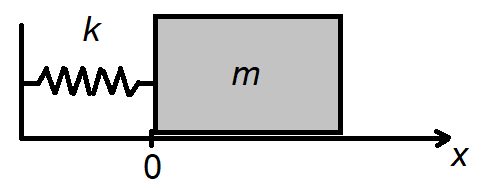
\includegraphics[width=0.5\linewidth]{screenshot001}
		\caption{Uma massa presa a uma mola}
		\label{fig:fig1}
	\end{figure}

	Lembramos que a Lei de Hooke nos diz que a força elástica é proporcional ao deslocamento em relação ao comprimento livre da mola, e é uma força restauradora. Assim, podemos escrever a componente da força ao longo do eixo $ x $ definido na figura como
	\begin{equation}\label{eq:eqFel}
		F_{el} = -kx
	\end{equation}

	\begin{parts}
		\part \label{part:q1a}  Escreva a Segunda Lei de Newton usando \ref{eq:eqFel} para o bloco e mostre que a equação diferencial que rege seu movimento é
		\begin{equation}\label{eq:odMov}
			\ddot{x} + \omega_0^{2}x=0
		\end{equation}
		para $ \omega_0=\sqrt{k/m} $.

		\begin{solution}
			Pela Segunda Lei de Newton:
			\[ F_r=m\,\ddot{x}\implies -k\,x=m\,\ddot{x}\implies \ddot{x}+\dfrac{k}{m}x=0\implies \ddot{x} + \omega_0^{2}\,x=0 \]

			\hfill\qedsymbol
		\end{solution}

		\clearpage

		\part \label{part:q1b}  Mostre que a função
		\begin{equation}\label{eq:elMovSol}
			x(t) = a\cos\omega_0 t + b\sin\omega_0 t
		\end{equation}
		é solução da equação diferencial \ref{eq:odMov}. Encontre as constantes $ a $ e $ b $ em termos das condições iniciais
		\[ x(0) = x_0,\quad \dot{x}(0) = v_0. \]

		\begin{solution}
			Derivando a equação \ref{eq:elMovSol}, temos:
			\[ \dot{x}(t)=-a\,\omega_0\sin\omega_0t+b\,\omega_0\cos\omega_0t \]

			e, derivando novamente:
			\[ \ddot{x}(t)=-a\,\omega_0^{2}\cos\omega_0t-b\,\omega_0^{2}\sin\omega_0t=-\omega_0^{2}\del{a\cos\omega_0 t + b\sin\omega_0 t}=-\omega_0^{2}\,x(t) \]

			Substuindo $ x(t) $ e $ \ddot{x}(t) $ em \ref{eq:odMov}, temos
			\begin{align*}
				\del{-\omega_0^{2}\,x(t)}+\omega_0^{2}\,x(t) & =0 \\
				0                                            & =0
			\end{align*}
			como queríamos verificar.

			Para encontrar $ a $ e $ b $, tomemos as condições iniciais:
			Para \ref{eq:elMovSol} em $ t=0 $:
			\begin{align*}
				x_0 & =x(0)                                           \\
				    & =a\,\cancelto{1}{\cos 0}+b\,\cancelto{0}{\sin0} \\
				a   & =x_0
			\end{align*}
			e, agora fazendo $ \dot{x}(0)=v_0 $:
			\begin{align*}
				v_0 & =\dot{x}(0)                                                          \\
				    & =-a\,\omega_0\,\cancelto{0}{\sin 0}+b\,\omega_0\,\cancelto{1}{\cos0} \\
				    & =b\,\omega_0                                                         \\
				b   & =\dfrac{v_0}{\omega_0}
			\end{align*}

		\end{solution}

		\part \label{part:q1c}  Utilizando a fórmula de cosseno da soma,
		\[ 	\cos(a+b) = \cos a\cos b - \sin a\sin b \]
		mostre que a solução \ref{eq:elMovSol} pode também ser escrita como
		\[ x(t) = A\cos(\omega_0 t - \phi) \]
		para $ A > 0 $ e $ \phi \in \intco{0,\num{2\pi}} $. Lembrando que a função $ \cos x $ têm período (constante $ \tau $ para qual a função se repete, $ f(x + \tau) = f(x) $ para todo $ x $) $ \num{2\pi} $, encontre o período $ \tau_0 $ da solução $ x(t) $. Escreva também sua frequência $ f_0 = 1/\tau_0 $, mostrando que $ \num{2\pi}f_0 = \omega_0 $. Por analogia ao movimento circular, chamamos então $\omega_0$ de frequência angular.

		\begin{solution}
			Seja $ A=\sqrt{a^{2}+b^{2}} $, devemos reescrever $ a=A\,\alpha $ e $ b=A\,\beta $, e como vale
			\[ \alpha^{2}+\beta^{2}=\del{\dfrac{a}{A}}^{2}+\del{\dfrac{b}{A}}^{2}=\dfrac{a^{2}+b^{2}}{A^{2}}=\dfrac{A^{2}}{A^{2}}=1 \]
			$ \alpha $ e $ \beta $ obedecem uma relação trigonométrica, e faremos $ \alpha:=\cos\phi $ e $ \beta:=\sin\phi $ para $ \phi\in\intco{0,\num{2\pi}} $.

			Daí, temos
			\begin{align*}
				x(t) & =a\cos\omega_0 t + b\sin\omega_0 t                            \\
				     & =A\,\alpha\cos\omega_0 t+A\,\beta\sin\omega_0t                \\
				     & =A\del{\cos\omega_0 t\cos\phi+\sin\omega_0t\sin\phi}          \\
				\intertext{dados $ \cos\phi=\cos(-\phi) $ e $ \sin(-\phi)=-\sin\phi $, podemos reescrever a expressão como}
				     & =A\del{\cos\omega_0t\cos(-\phi)-\sin\omega_0t\del{-\sin\phi}} \\
				     & =A\del{\cos\omega_0t\cos(-\phi)-\sin\omega_0t\sin(-\phi)}     \\
				     & =A\del{\cos\del{\omega_0t-\phi}}
			\end{align*}

			Nesse formato, podemos fazer:
			\begin{align*}
				x(t)                      & =x(t+\tau)                                                                \\
				A\cos\del{\omega_0t-\phi} & =A\cos\del{\omega_0\del{t+\tau}-\phi}                                     \\
				A\cos\del{\omega_0t-\phi} & =A\cos\del[0]{\omega_0t-\phi+\underbrace{\omega_0\,\tau}_{=\,\num{2\pi}}}
			\end{align*}
			daí, temos
			\begin{gather*}
				\omega_0\,\tau=2\pi\implies\tau=\dfrac{2\pi}{\omega_0}\\
				f_0=\dfrac{\omega_0}{2\pi}\implies 2\pi\,f_0=\omega_0
			\end{gather*}

			\hfill\qedsymbol
		\end{solution}

		\part \label{part:q1d} Suponha agora que colocássemos uma força constante $ F_0 $ agindo no bloco ao longo do eixo $ x $. Como se alterariam as equações \ref{eq:odMov} e \ref{eq:elMovSol}, e a frequência $ f_0 $? Dica: Considere uma substituição da forma $ y = x - X $, para $ X $ constante.

		\begin{solution}
			Pela Segunda Lei de Newton, temos
			\begin{align*}
				F_r                      & =m\,\ddot{x}    \\
				F_{el}+F_0               & =m\,\ddot{x}    \\
				-k\,x+F_0                & =m\,\ddot{x}    \\
				\ddot{x}+\dfrac{k}{m}\,x & =\dfrac{F_0}{m} \\
				\ddot{x}+\omega_0^{2}\,x & =\dfrac{F_0}{m}
			\end{align*}
			Fazendo $ y=x-X\implies \dot{y}=\dot{x}\implies\ddot{y}=\ddot{x} $, temos
			\begin{align*}
				\ddot{y}+\omega_0^{2}\,\del{y+X}         & =\dfrac{F_0}{m}                                 \\
				\ddot{y}+\omega_0^{2}\,y+\omega_0^{2}\,X & =\dfrac{F_0}{m}                                 \\
				\ddot{y}+\omega_0^{2}\,y                 & =\dfrac{F_0}{m}-\omega_0^{2}\,X\stackrel{!}{=}0
			\end{align*}
			E, daí, $ X=\dfrac{F_0}{m\,\omega_0^{2}} $. Portanto, \ref{eq:odMov} fica em função de $ y(t) $ e \ref{eq:elMovSol} terá forma \[ y(t)=x(t)-\dfrac{F_0}{m\,\omega_0^{2}} \]
			o que não altera sua frequência, pois corresponde à uma translação da solução, e não altera sua forma.
		\end{solution}

		\part \label{part:q1e} Substitua condições iniciais na solução que você encontrou em \ref{ques:q1}.\ref{part:q1d}. Escolha valores para $ m,k $ e faça alguns gráficos para diferentes valores de $ x_0, v_0, F_0 $. Pode ser a mão ou utilizando algum software, mas faça suficientes para que você consiga concluir coisas interessantes sobre o movimento.
		Anote aqui gráficos que você considera relevantes e suas observações e conclusões sobre eles.
	\end{parts}

	\bigskip

	\titledquestion{Modelando uma Corda Vibrante} \label{ques:q2}
	Agora que temos uma noção de que tipos de leis físicas geram um sistema oscilatório, e como elas se comportam de uma maneira genérica, nosso objetivo agora é modelar uma corda de violino em termos desse formalismo simplificado.

	Suponha que temos uma corda homogênea de massa $ M $ tensionada por uma tração $ T $, de comprimento $ L $ fixada em ambas as pontas. Uma análise ondulatória básica da situação nos diria que a velocidade de propagação das ondas nessa corda é $ c = \sqrt{TL/M} $, e que o comprimento de onda da oscilação fundamental é $ \lambda = 2L $. Assim, a frequência fundamental da corda seria
	\[ f_0=\dfrac{c}{\lambda}=\dfrac{1}{2L}\sqrt{\dfrac{TL}{M}}. \]

	Com isso, se quisermos modelar a corda como um oscilador harmônico, é imprescindível que
	sua frequência de oscilação livre seja reproduzida pelo oscilador simplificado que construímos, e portanto fixamos sua frequência angular como
	\begin{equation}\label{eq:angFreq}
		\omega_0=\num{2\pi}f_0=\pi\sqrt{\dfrac{T}{ML}}
	\end{equation}

	Vamos então a nosso modelo. Queremos estudar como a corda se comporta de acordo com a posição ao longo dela que aplicamos uma perturbação (no caso, a excitação pelo arco). Considere um fio leve de comprimento $ L $ preso a duas paredes paralelas, suponha que existe uma bolinha de massa $ m $ presa à uma distância $ rL $ da parede esquerda e $ (L - rL) $ da parede direita. Imagine que puxemos a massa para cima por uma distância $ x $ como exemplificado na figura \ref{fig:fig2}.

	\begin{figure}[H]
		\centering
		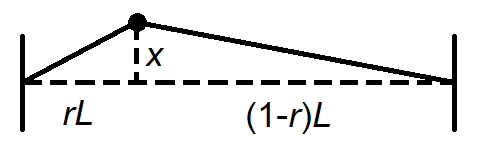
\includegraphics[width=0.5\linewidth]{screenshot002}
		\caption{Massa no fio deslocada}
		\label{fig:fig2}
	\end{figure}

	Supondo que as trações variam pouco nessa pequena distensão, a geometria do fio resultará numa força restauradora proporcional ao deslocamento.

	\begin{parts}
		\part \label{part:q2a}
		Encontre a constante elástica efetiva $ k $ agindo na massa em termos de $ T,L $ e $ r $. Você pode utilizar que, para ângulos pequenos em radiano, $ \sin\theta \approx \theta \approx \tan\theta $.

		\begin{solution}

			\begin{multi}
				Desenhando a situação, temos o esquema ao lado.

				Dado que $ t_1\approx t_2\approx T $, temos a força resultante sobre o corpo atuando na vertical, e daí, pela Segunda Lei de Newton
				\[ -T\sin\vartheta-T\sin\varphi=F_r=m\,\ddot{x} \]

				\nextcol

				\centering
				\begin{tikzpicture}[x=2cm,y=2cm, scale=1.5]
					\coordinate (O) at (0,0);
					\coordinate (A) at (30:0.9);
					\coordinate (B) at (2,0);

					\fill[pattern=north west lines] (-0.2,0.5) rectangle (0,-0.5);
					\fill[pattern=north west lines] (B)++(0,0.5) rectangle +(0.2,-1);
					\draw[dashed] (O) -- node[below] {$ r\,L $} (A|-O) -- node[below] {$ (1-r)L $} (B) (A) -- node[right] {$ x $} (A|-O);
					\draw[thick] (0,0.5) -- (0,-0.5) (B)++(0,0.5) -- +(0,-1);

					\draw (0,0) -- (A) -- (2,0);

					\draw[-Latex,red] (A) -- ($ (A)!0.25!(B) $) node[above] {$ t_1 $};
					\draw[-Latex,red] (A) -- ($ (A)!0.35!(O) $) node[above] {$ t_2 $};
					\filldraw (A) circle (1pt) node[above] {$ m $};

					\pic[draw=black, angle radius=20pt,angle eccentricity=1,"$ \vartheta $" {xshift=6pt,yshift=2pt}] {angle=B--O--A};

					\pic[draw=black, angle radius=25pt,angle eccentricity=1,"$ \varphi $" {xshift=-10pt,yshift=2pt}] {angle=A--B--O};
				\end{tikzpicture}
			\end{multi}

			Porém, sendo essa força elástica, podemos escrevê-la na forma
			\begin{equation}\label{eq:tFrKx}
				-T\sin\vartheta-T\sin\varphi=-k\,x
			\end{equation}
			para uma constante $ k\in\mathbb{R} $.

			Sendo
			\begin{gather*}
				\tan\vartheta=\dfrac{x}{r\,L}\implies x=r\,L\tan\vartheta\\
				\sin\vartheta\approx \tan\vartheta\\
				\sin\varphi \approx \tan\varphi=\dfrac{x}{(1-r)L}
			\end{gather*}
			isolando $ k $ em \ref{eq:tFrKx}, temos
			\begin{align*}
				k         & =\dfrac{T\sin\vartheta+T\sin\varphi}{r\,L\tan\vartheta}\approx-\dfrac{T\tan\vartheta+T\tan\varphi}{r\,L\tan\vartheta} \\[1ex]
				          & =\dfrac{T}{r\,L}\cdot\dfrac{\tan\vartheta+\tan\varphi}{\tan\vartheta}                                                 \\[1ex]
				          & =\dfrac{T}{r\,L}\cdot\dfrac{\dfrac{x}{r\,L}+\dfrac{x}{(1-r)L}}{\dfrac{x}{r\,L}}                                       \\[1ex]
				          & =\dfrac{T}{r\,L}\cdot\dfrac{\cancel{x}\del{\dfrac{(1-r)+r}{r(1-r)L}}}{\cancel{x}\dfrac{1}{r\,L}}                      \\[1ex]
				          & =\dfrac{T}{r\,L}\cdot\dfrac{r\,L}{r\,L(1-r)}                                                                          \\[1ex]
				\Aboxed{k & =\dfrac{T}{r(1-r)L}}
			\end{align*}

		\end{solution}

		\clearpage

		\part \label{part:q2b}
		Fixando a frequência angular $ \omega_0 $ dada em \ref{eq:angFreq}, mostre que a massa a ser escolhida para o oscilador ter a frequência certa é da forma
		\[ m=\eta\dfrac{M}{r(1-r)} \]
		e encontre a constante adimensional $ \eta $.

		\begin{solution}
			Tomando a expressão de $ k $ encontrada no item anterior, e tendo $ \omega_0=\sqrt{k/m} $, que deve igualar a frequência angular fixada, temos:
			\begin{align*}
				\omega_0                & =\sqrt{\dfrac{\dfrac{T}{r(1-r)L}}{m}}     \\
				\pi\sqrt{\dfrac{T}{ML}} & =\sqrt{\dfrac{T}{m\,r(1-r)L}}             \\
				\pi^{2}\dfrac{T}{ML}    & =\dfrac{T}{m\,r(1-r)L}                    \\
				m                       & =\dfrac{1}{\pi^{2}}\cdot\dfrac{M}{r(1-r)}
			\end{align*}
			portanto, $ \eta=1/\pi^{2} $.

			\hfill\qedsymbol
		\end{solution}
	\end{parts}

	Com isso, temos a capacidade de encapsular o movimento aproximado da corda em termos do seu comportamento no ponto de aplicação do arco, a uma distância $ rL $ do ponto de fixação. Só nos falta modelar o arco em si.

	\bigskip

	\titledquestion{A Excitação da Corda pelo Arco} \label{ques:q3}
	O modelo que vamos utilizar para o arco é o de uma barra infinita que se move com velocidade fixa e constante u para o sentido $ x > 0 $, aplicando uma força normal $ N $ na massa, com coeficientes de atrito estático e cinético $ \mu_s > \mu_k $. Adaptando o modelo da figura \ref{fig:fig1} temos uma nova representação na figura \ref{fig:fig3}.

	Vamos considerar que assim que o contato é estabelecido, a corda gruda no arco. Isto é, ela imediatamente ganha velocidade $ u $ e permanece com esta até o atrito não ser suficiente para segurar a força da mola.

	\begin{parts}
		\part \label{part:q3a} A corda ira permanecer grudada no arco até chegar em $ x = \Delta $. Encontre o valor de $\Delta$.
		Assim que a corda solta do arco, o sistema começará um movimento harmônico sujeito a uma força externa constante. Chame o instante de desprendimento de $ t_0 = 0 $.

		\begin{solution}
			Sendo $ F_{at\,s}=N\,\mu_s $ a força de atrito estático pela condição do problema, sabemos que $ x=\Delta $ quando $ |F_{el}|=|F_{at\,s}| $ e, portanto, temos:
			\[ k\,\Delta=N\,\mu_s\implies \Delta=\dfrac{N\,\mu_s}{k} \]
		\end{solution}

		\part \label{part:q3b} Escreva a Segunda Lei de Newton para o elemento de massa da corda. Encontre a equação diferencial que rege o movimento oscilatório da corda, e a correspondente solução em termos das condições iniciais $ x(0) = x 0 $ e $ \dot{x}(0) = v_0 $. Lembre-se do que você fez em \ref{ques:q1}.\ref{part:q1e}. Determine os valores de $ x_0 $ e $ v_0 $ em termos dos parâmetros dados.

		\begin{figure}[H]
			\centering
			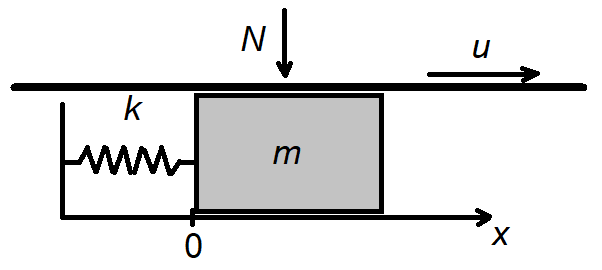
\includegraphics[width=0.5\linewidth]{screenshot003}
			\caption{Arco pressionando a corda}
			\label{fig:fig3}
		\end{figure}

		\begin{solution}
			Sendo $ F_{at\,k}=N\,\mu_k $ a força de atrito cinético, pela Segunda Lei de Newton, temos:
			\begin{align*}
				F_r                            & =m\,\ddot{x}                                                                                                   \\
				F_{el}+F_{at\,k}               & =m\,\ddot{x}                                                                                                   \\
				-k\,x+N\,\mu_k                 & =m\,\ddot{x}                                                                                                   \\
				\ddot{x}+\dfrac{k}{m}x         & =-\dfrac{N\,\mu_k}{m}                                                                                          \\
				%			\ddot{x}+\omega_0^{2}\,x&=-\dfrac{N\,\mu_k}{m}\\
				\intertext{pelo método de mudança de variáveis, tomando $ y=x-X $, temos:}
				\ddot{y}+\dfrac{k}{m}\del{y+X} & =-\dfrac{N\,\mu_k}{m}                                                                                          \\
				\ddot{y}+\dfrac{k}{m}y         & =-\dfrac{N\,\mu_k}{m}-\dfrac{k}{m}X\stackrel{!}{=}0\implies X=-\dfrac{N\,\mu_k}{k}=-\Delta\dfrac{\mu_k}{\mu_s}
			\end{align*}
			Daí, temos
			\begin{equation}\label{eq:genYform}
				y(t)=x(t)-X\implies y(t)=a\cos\omega_0t+b\sin\omega_0t+\Delta\dfrac{\mu_k}{\mu_s}
			\end{equation}

			Sendo $ y(0)=x_0=\Delta $ (pois a massa está nesse ponto em $ t_0 $) e $ \dot{y}(0)=v_0=u $ (pois a massa acabou de se desgrudar do arco), resolvendo \ref{eq:genYform} para $ t=0 $, temos:
			\[ y(0)=a\,\cancelto{1}{\cos\omega_0\cdot0}+b\,\cancelto{0}{\sin\omega_0\cdot0}+\Delta\dfrac{\mu_k}{\mu_s}=a+\Delta\dfrac{\mu_k}{\mu_s}=\Delta\implies a=\Delta\del{1-\dfrac{\mu_k}{\mu_s}} \]
			e derivando \ref{eq:genYform} e resolvendo para $ t=0 $, temos:
			\[ \dot{y}(0)=-a\,\omega_0\,\cancelto{0}{\sin\omega_0\cdot0}+b\,\omega_0\,\cancelto{1}{\cos\omega_0\cdot0}=\omega_0\,b=u\implies b=\dfrac{u}{\omega_0} \]

			Substituindo ambos em \ref{eq:genYform}, temos:
			\begin{equation}\label{key}
				y(t)=\del{\Delta-\dfrac{N\,\mu_k}{m\,\omega_0^{2}}}\cos\omega_0t+\dfrac{u}{\omega_0}\sin\omega_0t+\Delta\dfrac{\mu_k}{\mu_s}
			\end{equation}
		\end{solution}

		A partir deste instante inicial, o movimento harmônico seguirá até um instante $ t_1 $ em que a corda gruda novamente no arco.
		\part \label{part:q3c} Para que isso seja possível, temos duas condições a serem satisfeitas. Uma sobre a velocidade $ \dot{x}(t_1) $ e uma sobre a posição $ x(t_1) $. Escreva essas condições.

		\begin{solution}
			Sabemos que a velocidade deve igualar $ u $, assim como na condição inicial, pois somente assim a massa estará parada em relação ao arco --- condição necessária e suficiente para que $ F_{at\,s} $ atue.

			Para a posição, devemos ter $ |y(t)|<\Delta $, pois a partir de $ \Delta $ a massa se desprende do arco.
		\end{solution}
		\part \label{part:q3d} Utilize a condição na velocidade para encontrar $ t_1 $. Você pode fazer isso por métodos gráficos ou algébricos. Para fazer na álgebra é interessante conhecer as fórmulas de arco duplo
		\begin{gather*}
			\sin 2\theta = 2\sin\theta\cos\theta,\\
			\cos 2\theta = \cos^{2} \theta - \sin^{2}\theta.
		\end{gather*}
		Mostre que a condição sobre a posição é imediatamente satisfeita.

		\begin{solution}
			Pela condição da velocidade, temos:
			\begin{align}
				\dot{y}(t_1)                                                            & =u\nonumber                                                                                                                          \\
				-a\,\omega_0\sin\omega_0t_1+u\cos\omega_0t_1                            & =u\quad\text{onde $ a=\Delta\del{1-\dfrac{\mu_k}{\mu_s}} $} \nonumber                                                                \\
				-a\,\omega_0\sin\omega_0t_1                                             & =u\del{1-\cos\omega_0t_1}\nonumber                                                                                                   \\
				\intertext{pelas fórmulas do arco duplo:}
				-a\,\omega_0\del{2\sin\dfrac{\omega_0t_1}{2}\cos\dfrac{\omega_0t_1}{2}} & =u\del{1-\del{\cos^{2}\dfrac{\omega_0t_1}{2}-\sin^{2}\dfrac{\omega_0t_1}{2}}}\nonumber                                               \\
				\intertext{pela relação fundamental da trigonometria:}
				-a\,\omega_0\cos\dfrac{\omega_0t_1}{2}\del{2\sin\dfrac{\omega_0t_1}{2}} & =u\del[2]{\underbrace{1-\cos^{2}\dfrac{\omega_0t_1}{2}}_{=\,\sin^{2}\dfrac{\omega_0t_1}{2}}+\sin^{2}\dfrac{\omega_0t_1}{2}}\nonumber \\
				-a\,\omega_0\cos\dfrac{\omega_0t_1}{2}\del{2\sin\dfrac{\omega_0t_1}{2}} & =u\sin\dfrac{\omega_0t_1}{2}\del{2\sin\dfrac{\omega_0t_1}{2}} \label{eq:t1par}
			\end{align}

			porém, para dividir por $ 2\sin\dfrac{\omega_0t_1}{2} $ em ambos os lados, devemos ter
			\[ 2\sin\dfrac{\omega_0t_1}{2}\neq 0\implies
				\sin\dfrac{\omega_0t_1}{2}\neq \sin n\pi \implies t_1\neq \dfrac{2n\pi}{\omega_0}=\tau\quad\text{para $ n\in\mathbb{N} $,} \]
			onde $ \tau $ é o período da função.

			Como $ y(0)=y(\tau)=\Delta $, devemos ter $ y(t)\neq\Delta $, e como $ \pm\Delta $ são valores extremos de $ y(t) $, devemos ter $ |y(t)|<\Delta $, que é a condição para a posição encontrada no item anterior.

			Dada a condição de posição, retomemos a resolução de \ref{eq:t1par}, temos:
			\begin{align}
				-a\,\omega_0\cos\dfrac{\omega_0t_1}{2} & =u\sin\dfrac{\omega_0t_1}{2}\nonumber                                                                             \\
				\intertext{tomando $ t_1\neq n\dfrac{\pi}{\omega_0} $:}
				-\dfrac{a\,\omega_0}{u}                & =\dfrac{\sin\dfrac{\omega_0t_1}{2}}{\cos\dfrac{\omega_0t_1}{2}}\nonumber                                          \\
				\tan\dfrac{\omega_0t_1}{2}             & =-\dfrac{a\,\omega_0}{u}\label{eq:tant1}                                                                          \\
				\dfrac{\omega_0t_1}{2}                 & =n\pi+\arctan\del{-\dfrac{a\,\omega_0}{u}}\nonumber                                                               \\
				\intertext{substituindo $ a $ de volta, temos}
				t_1                                    & =\dfrac{2}{\omega_0}\del{n\pi+\arctan\del{-\del{\Delta\del{1-\dfrac{\mu_k}{\mu_s}}}\dfrac{\omega_0}{u}}}\nonumber \\
				\Aboxed{t_1                            & =\dfrac{2}{\omega_0}\del{n\pi+\arctan\del{\dfrac{\Delta\,\omega_0}{u}\del{\dfrac{\mu_k}{\mu_s}-1}}}}\nonumber
			\end{align}
		\end{solution}

		Quando a corda gruda no arco, ela irá desprender novamente quando o sistema finalmente chega em $ x = \Delta $. Isso ocorre no instante $ t_2 $. A partir daí o movimento irá começar a se repetir.

		\part \label{part:q3e} Encontre $ t_2 $ em termos de parâmetros dados e $ t_1 $. Utilize isso e o resultado de \ref{ques:q3}.\ref{part:q3d} para	escrever a frequência $ f $ do movimento em termos só de parâmetros dados. Esboce um gráfico do movimento periódico do ponto da corda.

		\begin{solution}
			Resolvendo $ y(t_2)=\Delta $, temos:
			\begin{align*}
				\Delta\del{1-\dfrac{\mu_k}{\mu_s}}\cos\omega_0t_2+\dfrac{u}{\omega_0}\sin\omega_0t_2+\Delta\dfrac{\mu_k}{\mu_s} & =\Delta                                                                                   \\
				a\cos\omega_0t_2-a                                                                                              & =-\dfrac{u}{\omega_0}\sin\omega_0t_2\quad\text{onde }a=\Delta\del{1-\dfrac{\mu_k}{\mu_s}} \\
				a\del{\cos\omega_0t_2-1}                                                                                        & =-\dfrac{u}{\omega_0}\sin\omega_0t_2                                                      \\
				\intertext{pelas fórmulas do arco duplo}
				a\del{\del{\cos^{2}\dfrac{\omega_0t_2}{2}-\sin^{2}\dfrac{\omega_0t_2}{2}}-1}                                    & =-\dfrac{u}{\omega_0}\del{2\sin\dfrac{\omega_0t_2}{2}\cos\dfrac{\omega_0t_2}{2}}          \\
				a\del{-\del{1-\cos^{2}\dfrac{\omega_0t_2}{2}}-\sin^{2}\dfrac{\omega_0t_2}{2}}                                   & =-\dfrac{u}{\omega_0}\del{2\sin\dfrac{\omega_0t_2}{2}\cos\dfrac{\omega_0t_2}{2}}          \\
				a\del{-2\sin^{2}\dfrac{\omega_0t_2}{2}}                                                                         & =-\dfrac{u}{\omega_0}\del{2\sin\dfrac{\omega_0t_2}{2}\cos\dfrac{\omega_0t_2}{2}}
			\end{align*}
			para $ t_2\neq n\dfrac{\pi}{\omega_0} $ e $ \dfrac{\mu_k}{\mu_s}\neq1 $:
			\begin{align*}
				\dfrac{\sin\dfrac{\omega_0t_2}{2}}{\cos\dfrac{\omega_0t_2}{2}} & =\dfrac{u}{\omega_0\,a}                                                \\
				\tan\dfrac{\omega_0t_2}{2}                                     & =-\del{\del{-\dfrac{u}{\omega_0\,a}}^{-1}}^{-1}                        \\
				\intertext{substituindo \ref{eq:tant1}, temos}
				                                                               & =-\del{\tan\dfrac{\omega_0t_1}{2}}^{-1}                                \\
				t_2                                                            & =\dfrac{2}{\omega_0}\del{n\pi-\arctan\del{\cot\dfrac{\omega_0t_1}{2}}} \\
			\end{align*}

			Como $ t_2 $ é o tempo que leva para a massa retornar à posição inicial, temos $ \tau=t_2\implies f=1/t_2 $, e, portanto:
			\[ f=\del{\dfrac{2}{\omega_0}\del{n\pi-\arctan\del{\cot\dfrac{\omega_0t_1}{2}}}}^{-1} \]
		\end{solution}

		\part \label{part:q3f}  Sendo $ f_0 = \omega_0/\num{2\pi} $ a frequência livre da corda, mostre que
		\[ \dfrac{f}{f_0}=\del{1+\dfrac{\alpha-\arctan\alpha}{\pi}}^{-1} \]
		onde $\alpha$ é uma função adimensional de parâmetros dados. Encontre $\alpha$ e esboce um gráfico da razão das frequências em termos de $\alpha$.

		\begin{solution}
			Fazendo
			\begin{align*}
				\dfrac{f}{f_0} & =\dfrac{\del{\dfrac{2}{\omega_0}\del{n\pi-\arctan\del{\cot\dfrac{\omega_0t_1}{2}}}}^{-1}}{2\pi/\omega_0}                \\
				               & =\del{\dfrac{2}{\omega_0}\del{n\pi-\arctan\del{\cot\dfrac{\omega_0t_1}{2}}}}^{-1}\cdot\del{\dfrac{2\pi}{\omega_0}}^{-1} \\
				               & =\del{\dfrac{4\pi}{\omega_0^{2}}\del{n\pi-\arctan\del{\cot\dfrac{\omega_0t_1}{2}}}}^{-1}
			\end{align*}

			Desisto :(.
		\end{solution}

		\part \label{part:q3g}  Para um violino e arco bem regulados, valores típicos para os atritos são de $ \mu_s = \num{1,1} $ e $ \mu_k = \num{0,4} $, e consideramos agora a corda Lá, de frequência livre $ f_0 = \SI{440}{\hertz} $. Estime outros valores necessários para construir gráficos de $ \alpha $ sobre a variação dos outros parâmetros. Discuta a sensibilidade da frequência sobre a variação destes.
	\end{parts}
\end{questions}
\end{document}
